% ============================================================
% 片段：s05c  对应原文 section3.tex 第 409--541 行；PDF 第 61--66 页
% 内容：§5.5--5.8（物理诠释、带 't Hooft 反常的规范化、弱 n-群、非可逆对称性一瞥）+ 致谢
% 译者：lead   审校状态：初稿
% ============================================================

% ==== 原文 PDF 第 61 页 ====
\subsection{物理诠释}
\label{sec:2-group-phys}

本节将说明 2-群如何描述物理系统中的高对称性结构。我们将导出 $\Pi_1$ 如何描述 $0$-形式对称性、$\Pi_2$ 如何描述 $1$-形式对称性，以及 $\alpha$、$\beta$ 如何描述二者如何结合。

现在用拓扑缺陷网络的观点来看上述结构。$\alpha$ 可理解为 $0$-形式缺陷（$\Pi_1$-缺陷）对与之相交的 $1$-形式缺陷（$\Pi_2$-缺陷，维数低一维）的扭曲：
\begin{center}
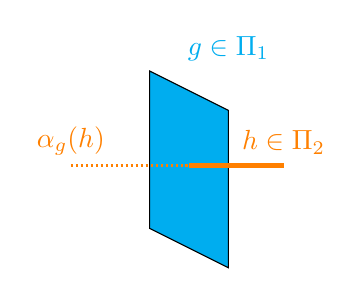
\begin{tikzpicture}
    \draw [yslant = -0.5, fill = cyan] (0,0) rectangle (1,2) (1,2.5)node[above , cyan] {$g\in\Pi_1 $};
    \draw[densely dotted, thick, orange] (-1,0.8) node[anchor = south] {$\alpha_{g}(h)$} -- (0.5,0.8)  ;
    \draw[ultra thick, orange] (0.5,0.8) -- (1.7,0.8) node[anchor = south]{$h\in \Pi_2$};
\end{tikzpicture}
\end{center}
穿过 $0$-形式对称性的生成元 $U_g$ 之后，$1$-形式对称性元素按 $h\mapsto \alpha_g(h)=g\rhd h$ 改变。

$\beta$ 的信息则编码在 $1$-形式缺陷的融合之中。
\begin{center}
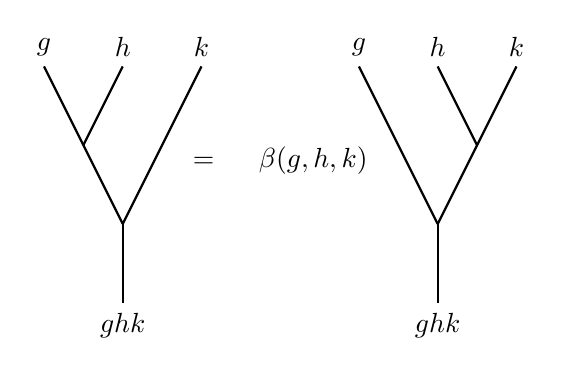
\begin{tikzpicture}[scale = 0.5]
    \draw[thick] (0,0) -- (2,-4) (0,0) node[above] {$g$};
    \draw[shift = {(8,0)} ,thick] (0,0) -- (2,-4) (0,0) node[above] {$g$};
    \draw[thick] (4,0) -- (2,-4) (4,0) node[above]{$k$}; 
    \draw[shift = {(8,0)}, thick] (4,0) -- (2,-4) (4,0) node[above]{$k$}; 
    \draw[thick] (2,-4) -- (2,-6) (2,-6) node[below]{$ghk$};
    \draw[shift = {(8,0)}, thick] (2,-4) -- (2,-6) (2,-6) node[below]{$ghk$};
    \draw[thick] (2,0) -- (1,-2) (2,0) node[above]{$h$};
    \draw[thick] (10,0) -- (11,-2) (10,0) node[above]{$h$} (6,-3) node[above]{$= \ \ \ \ \beta(g,h,k)$} ;
    
\end{tikzpicture}
\end{center}

上述从左到右的过程，按照共形场论中融合规则的叫法，有时称为 F-移动（F-move）。经过一次 F-移动之后，会出现 $1$-形式对称性的一个新生成元 $\beta(g,h,k)$。

弱 2-群的背景规范场为：$0$-形式对称性的 $A$ 与 $1$-形式对称性的 $B$。用单纯集（平坦联络）的语言来说，
\begin{enumerate}
    \item 对 $0$-形式部分，跃迁函数 $A_{ij}\in C^1(M,\Pi_1)$，而 $1$-上闭链条件要求对每个 2-单纯形 $\{ ijk\}$ 有
    \be A_{ij}A_{jk}A_{ki} = {\rm id}_{\Pi_1}  \ee
    
    \item 对 $1$-形式部分，规范场 $B\in C^2(M,\Pi_2)$ 满足一个扭曲-平移的上闭链条件
    \be\ba
    \delta_A B &= A^* \beta \\
    \Leftrightarrow \alpha_{A_{ij}} (B_{jkl}) B_{ikl}^{-1} B_{ijl} B_{ijk}^{-1} &= \beta(A_{ij},A_{jk},A_{kl})
    \ea\ee
    称之为“扭曲的”，是因为微分 $\delta_A$ 比通常的 Čech 微分 $\delta$ 多了一个 $\Pi_1$-作用；称之为“平移的”，是因为它不等于 0，而是等于 Postnikov 不变量。
\end{enumerate}

规范变换应当保持平坦性条件。这里有两类规范变换：
\begin{enumerate}
    \item 第一类是
    \be A \mapsto A , \ \ B\mapsto B + \delta_A \Lambda  \ee
    $A$ 场保持不变，$B$ 被平移一个扭曲恰当项。
    \item 第二类更为复杂，
    \be\ba 
    A_{ij} &\mapsto A^f_{ij} = f_i A_{ij} f_j^{-1} \\   
    B&\mapsto \alpha_f(B) + \xi(A,f) , \\ 
    \xi(A,f) \in C^2(M,\Pi_2) \ \ &{\rm and} \ \delta_{A^f}\xi(A,f) = A^{f*} B-\alpha_f (A^*\beta) \ .
    \ea\ee
\end{enumerate}

\begin{yizhu}
式 $\delta_A B = A^*\beta$ 的扭曲-平移条件极易写错符号与次序：展开为
$\alpha_{A_{ij}}(B_{jkl})B_{ikl}^{-1}B_{ijl}B_{ijk}^{-1}=\beta(A_{ij},A_{jk},A_{kl})$，
其中 $\alpha_{A_{ij}}(B_{jkl})$ 表示 $\Pi_1$ 通过 $\alpha$ 作用在 $\Pi_2$ 上（即交叉模的 Peiffer 作用）。
核对时请注意：$\delta_A$ 的下标 $A$ 指用 $0$-形式联络 twist 通常的 Čech 微分；若把 $\alpha$ 的作用方向记反，
得到的 Postnikov 类会差一个逆。
\end{yizhu}

\begin{yizhu}
第二类规范变换中的 $\xi(A,f)$ 不是自由参数：它必须满足 $\delta_{A^f}\xi = A^{f*}B-\alpha_f(A^*\beta)$，
这正是“平坦性在规范变换下保持”的要求。作者未展开此式的推导；其实质是：$B\mapsto \alpha_f(B)+\xi$ 之后，
要求 $\delta_{A^f}B'=A^{f*}\beta$，再与 $\delta_{A^f}\alpha_f(B)$ 的定义比较即得。
\end{yizhu}

% ==== 原文 PDF 第 62 页 ====
凝聚态系统中自然出现的 2-群结构之一是“对称性富化的规范理论”（symmetry-enriched gauge theory），
它可以看作对称性富化拓扑（SET）态的特例\cite{etingof2010fusion,PhysRevB.87.155115,PhysRevB.87.165107,Chang_2015,PhysRevB.93.155121,PhysRevB.94.235136,PhysRevB.96.115107,PhysRevB.100.115147,10.21468/SciPostPhys.8.2.028,PhysRevB.106.115104}。

例如，考虑一个 $(2+1)$ 维系统，其阿贝尔规范群为 $A$、对称群为 $\Pi_1$。$A$ 规范理论的任意子（激发）由规范群 $A$ 的量子双重（quantum double）描述。在阿贝尔情形，这对应于 $A\times\hat{A}$，其中 $A$ 与 $\hat{A}=\text{Hom}(A,U(1))$ 分别描述 $A$ 规范理论中的规范通量与规范荷。这类任意子的世界线可理解为 $1$-形式对称性 $\Pi_2=A\times\hat{A}$ 的拓扑缺陷线（TDL）。另一方面，$0$-形式对称性 $\Pi_1$ 正是通过作用 $\alpha$ 作用在任意子上。

2-群理论的全部数据与相容性条件，都可追溯到 SET 态的分类数据与障碍\cite{etingof2010fusion,PhysRevB.100.115147,wang2021domain}。更一般地，若考虑非阿贝尔的 $A$，则作为 $1$-形式对称性的量子双重 $\Pi_2=DA$ 将是非可逆的。于是 SET 态将对应于具有非可逆 $1$-形式对称性与可逆 $0$-形式对称性的系统；这两类对称性的相互作用会使分类变得更加复杂\cite{etingof2010fusion,PhysRevB.100.115147}。2-规范理论的格点模型可以写成离散非线性 $\sigma$-模型，这一表示来自把时空三角剖分为与 2-群相伴的分类空间，详见文献~\cite{PhysRevB.100.045105}。

% ==== 原文 PDF 第 63 页 ====
\subsection{例：带 't Hooft 反常的规范化}
\label{sec:2-group-gauging}

这里给出弱 2-群对称性的一个物理应用。

考虑一个 3 维量子场论，其 $0$-形式整体对称为 $\hat{\Pi}_2\times \Pi_1$，其中暂时取 $\hat{\Pi}_2$ 为阿贝尔群。该系统具有由下式描述的混合 't Hooft 反常：
\be S = 2\pi \int_{M_4} C\cup A^*\beta  \ee
其中 $C$ 是 $\hat{\Pi}_2$ 的背景 $1$-形式规范场，$A$ 是 $\Pi_1$ 的背景 $1$-形式规范场，$\beta$ 是 Postnikov 类。存在 't Hooft 反常时，我们无法对完整的 $\hat{\Pi}_2\times \Pi_1$ 对称性作规范化；但在对 $\hat{\Pi}_2$ 作规范化之后，可以得到一个新的 $1$-形式对称性 $\Pi_2\cong {\rm Hom}(\hat{\Pi}_2,U(1))$ 及相应的 $2$-形式背景规范场 $B$。

完成上述步骤后，新的拓扑作用量为
\be S = 2\pi \int_{M_3} C\cup B  + 2\pi \int_{M_4} C\cup A^*\beta \ee
它应当在 $\Pi_2$ 规范变换下规范不变，于是要求
\be  \delta B + A^* \beta = 0 \ee
这与我们先前给出的弱 2-群定义一致（若仔细看，会差一个符号约定）。因此在该理论中，$\Pi_1$、$\Pi_2$ 构成一个 2-群对称性 $(\Pi_1,\Pi_2,1,\beta)$，其中 $1$ 表示平凡作用。

\begin{yizhu}[原文疑误]
作者在此明言“差一个符号约定”（up to a sign notation, if you watch carefully），但未说明符号来源。
通常的约定是 $\delta B + A^*\beta = 0$ 与 $\delta_A B = A^*\beta$ 之间相差 $B\mapsto -B$ 的重新定义；
两种写法描述的 2-群相同，但若与文献直接比对公式，须先统一 $B$ 的符号约定。
\end{yizhu}

% ==== 原文 PDF 第 64 页 ====
\subsection{推广：弱 $n$-群}
\label{sec:n-group}
正如前面所说，“相等”这一条件总可以放松为“等价”，而描述这种等价关系所用的语言各有不同。

我们当然可以想象弱 $n$-群的草图：存在 $n$-态射，用来填补具有相同源与靶的两个 $(n-1)$-态射之间的空隙，如此逐级下降直到 $1$-态射。不过这里我们想描述的是一个相对简单的情形，它只是前一个例子的平凡推广。

回忆命题~\ref{prop:gauge}：当我们对一个 $p$-形式对称性作规范化时，将得到一个 $(d-p-2)$-形式对称性。现在考虑在 $(n+1)$ 维时空中、对完整的 $\hat{\Pi}_2\times \Pi_1$ 中的 $0$-形式对称性 $\hat{\Pi}_2$ 作规范化，设 't Hooft 反常用
\be  S = 2\pi \int_{M_{n+2}} C\cup A^*\beta   \ee
描述，其中 $\beta\in H^{n+1}(\Pi_1,\Pi_2)$ 是 Postnikov 类。这一特殊版本的弱 $n$-群中，$\Pi_1$ 是描述 $1$-态射的 $0$-形式对称性，$\Pi_2$ 是描述 $n$-态射的 $(n-1)$-形式对称性。

\subsection{非可逆对称性一瞥}
\label{sec:non-invertible}
本讲义中遇到的广义对称性都是可逆对称性，可以用群或高群描述。更广泛的一类对称性是非可逆对称性，其中包括更一般的高阶范畴对称性。对这类对称性，拓扑生成元服从一般的融合规则
\be
U_g(M)U_h(M)=\sum_i U_{g_i}(M_i)
\ee
而不是群的结合律。注意右端甚至可以由定义在维数各不相同的流形 $M_i$ 上的拓扑算符组成。非可逆对称性的研究领域发展迅速，感兴趣的读者可参阅近期讲义\cite{Schafer-Nameki:2023jdn}。

从凝聚态物理的角度看，$2+1$ 维拓扑序中非阿贝尔任意子的产生算符，可以解释为非可逆对称性的生成元。该对称性能够作用在 $1+1$ 维边界上，从而对可能的边界理论施加非可逆的对称性约束\cite{PhysRevResearch.2.043086,kong_mathematical_2020,kong_mathematical_2021,PhysRevResearch.2.033417,ji2022unified,PhysRevB.107.155136,PhysRevB.108.075105}。

我们给出 $d$ 维 $Spin(4N)$ 杨–米尔斯理论的一个例子\cite{Bhardwaj:2022yxj}。该理论具有 $\mb{Z}_2^{(1)}\times\mb{Z}_2^{(1)}$ 的 $1$-形式中心对称性，其背景 $2$-形式规范场记为 $B_2$ 与 $C_2$；此外还有 $D_{2N}$ 根系的一个 $\mb{Z}_2^{(0)}$ 外自同构，其背景规范场为 $A_1$。$\mb{Z}_2^{(0)}$ 对称性作用在 $D_{2N}$ 的 Dynkin 图上为

\begin{center}
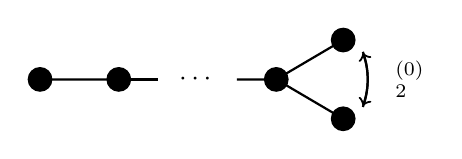
\begin{tikzpicture}
    \filldraw[] (0,0) circle (0.15) (1,0) circle (0.15) (3,0) circle (0.15) (3.85,0.5) circle (0.15) (3.85,-0.5) circle (0.15);
    \draw[thick] (0,0)--(1,0) (2.5,0)--(3,0) (3,0)--(3.85,0.5) (3,0)--(3.85,-0.5);
    \draw[thick] (1,0)--(1.5,0) node[anchor = west]{\textbf{$ \ \cdots$}};
    \draw[thick,->] (4.1,-0.35) arc (-20:20:1);
    \draw[thick,->] (4.1,0.35) arc (20:-20:1);
    \node[] at (4.7,0){$\bbZ_2^{(0)}$};
\end{tikzpicture}
\end{center}
它把 $D_{2N}$ 的表示 $\mbf{R}$ 映为其复共轭表示 $\overline{\mbf{R}}$。现在，在以 $B_2$ 为背景规范场对 $\mb{Z}^{(1)}$ 对称性作规范化之后，我们得到 $SO(4N)$ 杨–米尔斯理论，其混合 't Hooft 反常为
\be
\mc{A}=\pi\int_{M_{d+1}} A_1\cup C_2\cup \hat{B}_{d-2}
\ee
其中 $\hat{B}_{d-2}$ 是 $(d-3)$-形式对偶对称性的背景规范场。

最后，若进一步对 $A_1$ 与 $\hat{B}_{d-2}$ 作规范化，我们将得到带非可逆对称性缺陷的 $Pin^+(4N)$ 理论。

一般而言，若一个非可逆对称性来自这类部分规范化，则称为\textbf{非内禀的非可逆对称性}（non-intrinsically non-invertible symmetry）；否则称为\textbf{内禀的非可逆对称性}（intrinsically non-invertible symmetry）。

\begin{yizhu}
本节的 $Spin(4N)$ 例子是“非内禀非可逆对称性”的标准范例：它来自对 $SO(4N)$ 理论的 $\mathbb{Z}_2^{(1)}\times\mathbb{Z}_2^{(1)}$ 中心对称性作部分规范化。核对时请注意：
$\hat{B}_{d-2}$ 是 $(d-3)$-形式对偶对称性的背景场，其形式次数为 $d-2$，与 $A_1\cup C_2$（$1+2=3$ 次）相乘后总次数为 $d+1$，恰好是 $M_{d+1}$ 上的反常作用量所要求的次数。
\end{yizhu}

% ==== 原文 PDF 第 65--66 页 ====
\section*{致谢}

我们感谢 Lakshya Bhardwaj、Chi-Ming Chang、Max Hubner、Ruizhi Liu、Sakura Schafer-Nameki、Fajie Wang、Jingxiang Wu 与 Yi Zhang 就相关课题的讨论。我们也感谢北京大学听众的讨论与提问。QRW 由中国国家自然科学基金资助（批准号 12274250）。YNW 由中国国家自然科学基金（批准号 12175004）、北京大学启动经费（批准号 7100603667）以及中国科协青年人才托举工程（2022QNRC001）资助。
